
\section{Simulation Details}
\label{sec:simulation}

In order to study jet images in a realistic scenario, we use Monte Carlo (MC) simulations of high energy particle collisions. One important jet tagging task is to distinguish the hadronic decays of high $p_T$ $W$ bosons from generic SM background processes computes of quarks and gluons.  To simulate high $p_T$ $W$ bosons, a hypothetical $W'$ boson is generated and forced to decay to a hadronically decaying $W$ boson and a $Z$ boson which decays invisibly.


Two physics processes are generated using \textsc{Pythia} 8.170~\cite{Pythia8,Pythia} at $\sqrt{s}=14$ TeV.   To simulate high $p_T$ hadronic $W$ decays, $W'$ bosons are generated to decay exclusively into a $W(\rightarrow qq')$ and $Z(\rightarrow\nu\nu)$.  The $p_T$ scale of the hadronically decaying $W$ is set by the mass of the $W'$ which is tuned to 600 and 800~GeV for this study so that the $200$ GeV $\lesssim p_T^W \lesssim 400$ GeV. In this $p_T^W$ range, the $W$ decay products are expected to merge within a cone of $R~1.0$ where $\Delta R^2=\Delta\phi^2+\Delta\eta^2\sim 4m_W^2/p_{T,W}^2$.  To study the impact on signal versus background, QCD dijets are generated with a range of $\hat{p}_T$ that is approximately in the same range as the relevant signal process.  Anti-$k_t$ jets are clustered using \textsc{FastJet}~\cite{fastjet} 3.0.3.  The signal processes are chosen such that jets with radius parameter $R = 1$ are most appropriate in capturing the decay products of the heavy particles.  The anti-$k_t$ jets are trimmed~\cite{trimming} by re-clustering the constituents into $R=0.3$ $k_t$ subjets and dropping those which have $p_T^\text{subjet}<0.05\times p_T^\text{jet}$. 

To model the discretization and finite acceptance of a real detector, a calorimeter of towers with size $0.1\times 0.1$ in $(y,\phi)$ extends out to $y=5.0$.  The total energy of the simulated particles incident upon a particular cell are added as scalars and the four-vector $p_j$ of any particular tower $j$ is given by

\begin{align}
\label{eq:calo}
p_j = \sum_{i\text{ incident on $j$}}E_i(\cos\phi_j/\cosh y_j,\sin\phi_j/\cosh y_j,\sinh y_j/\cosh y_j,1).
\end{align}


\begin{figure}[bt]
  \begin{center}
      \subfloat[Unweighted $p_T$ distribution \label{subfig:unweighted_pt}]{
        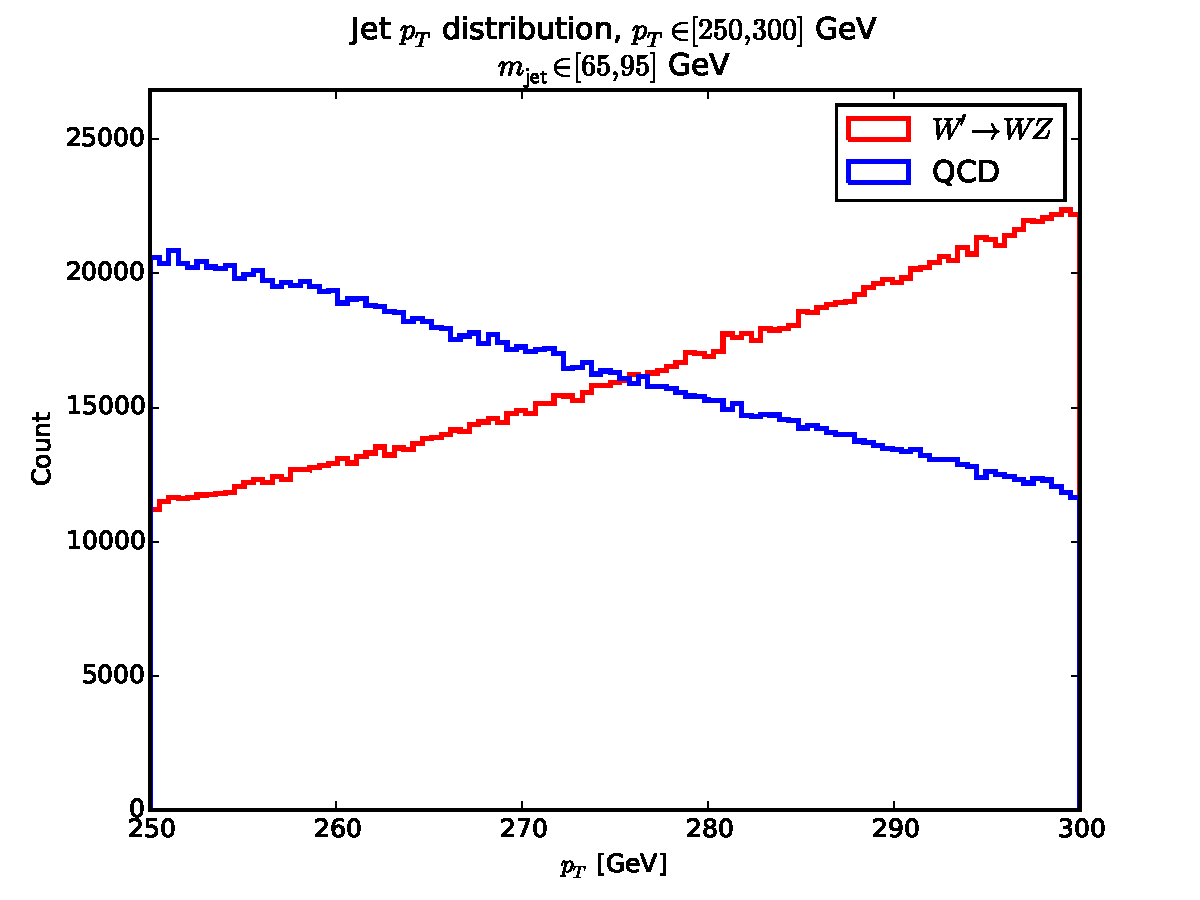
\includegraphics[width=0.5\textwidth]{figures/unweighted-pt-distribution-[250-300].pdf}
      }
      \subfloat[Weighted $p_T$ distribution \label{subfig:weighted_pt}]{
        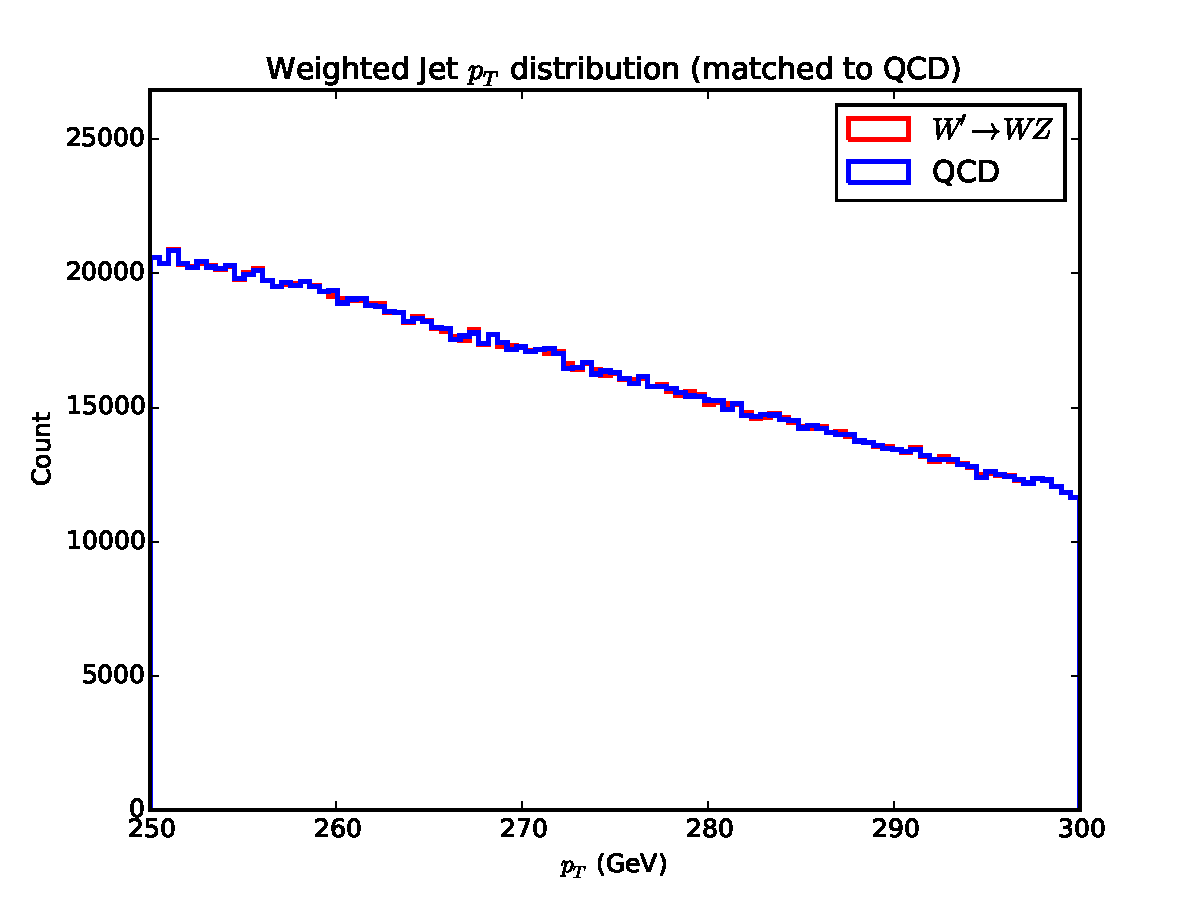
\includegraphics[width=0.5\textwidth]{figures/weighted-pt-distribution[250-300].pdf}
      }
      \caption{ Jets originating from the $W'\rightarrow WZ$ decay are re-weighted such that their $p_T$ spectrum matches that of QCD jets\label{fig:pt} }
    \end{center}
\end{figure}


\begin{figure}[bt]
  \begin{center}
  
  
      \subfloat[Weighted jet mass distribution \label{subfig:weighted_mass}]{
        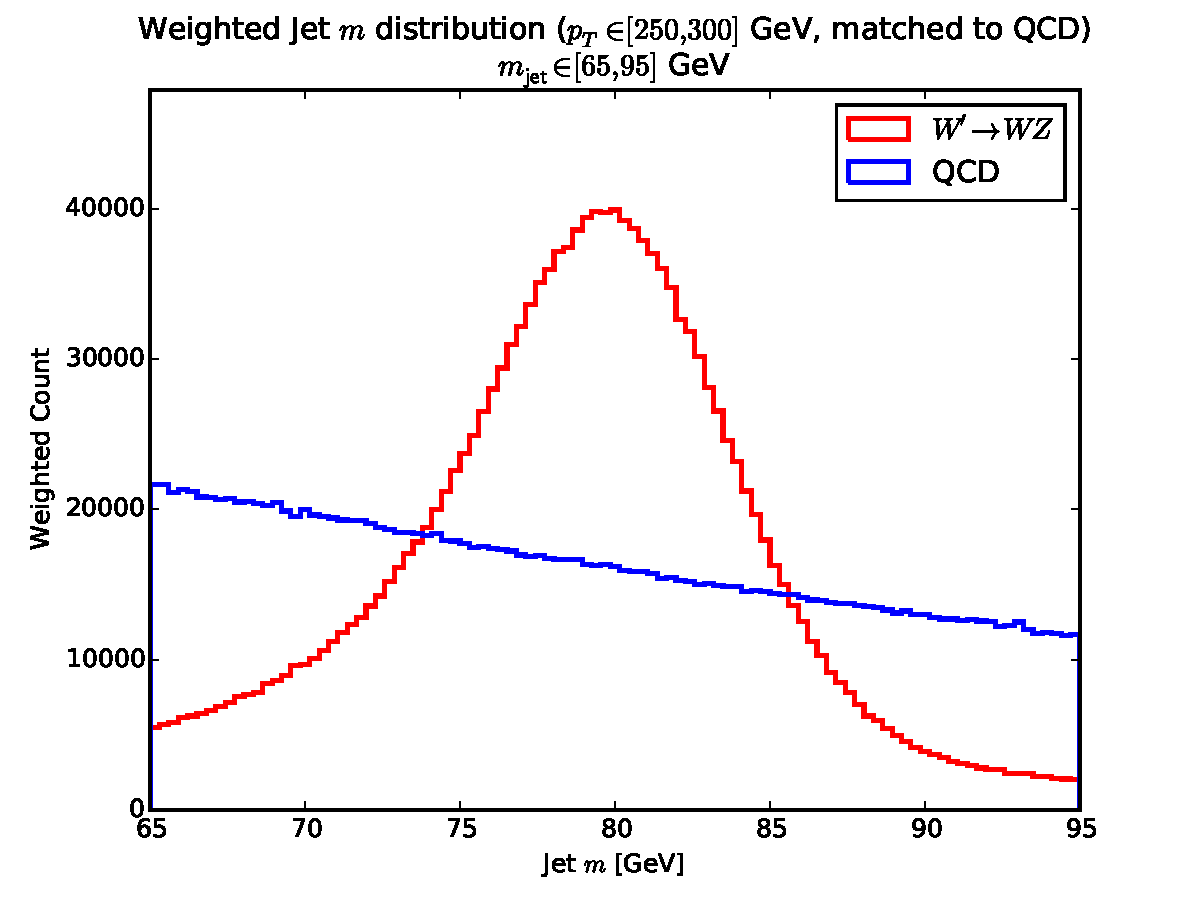
\includegraphics[width=0.5\textwidth]{figures/weighted-mass-distribution[250-300].pdf}
      }
      \subfloat[Weighted $\tau_{21}$ distribution \label{subfig:weighted_nsj}]{
        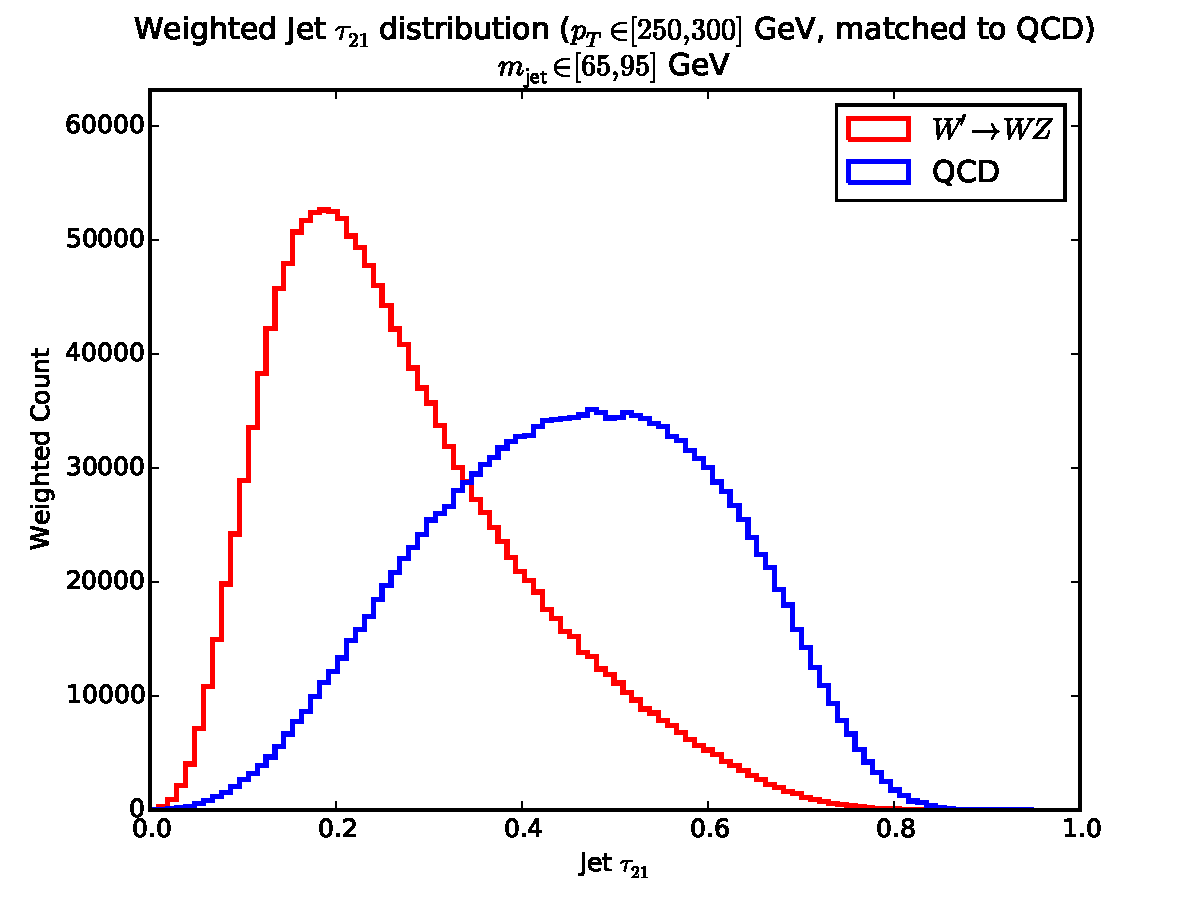
\includegraphics[width=0.5\textwidth]{figures/weighted-tau21-distribution[250-300].pdf}
      }
      \caption{Weighted mass (left) and $n$-subjettiness (right) of samples, with $W'\rightarrow WZ$ decays in red and QCD jets in blue.\label{fig:mass_nsj_spectrum} }
    \end{center}
\end{figure}  



\begin{figure}[bt]
  \begin{center}
  
      \subfloat[Average weighted $W'\rightarrow WZ$ image \label{subfig:weighted_sig}]{
        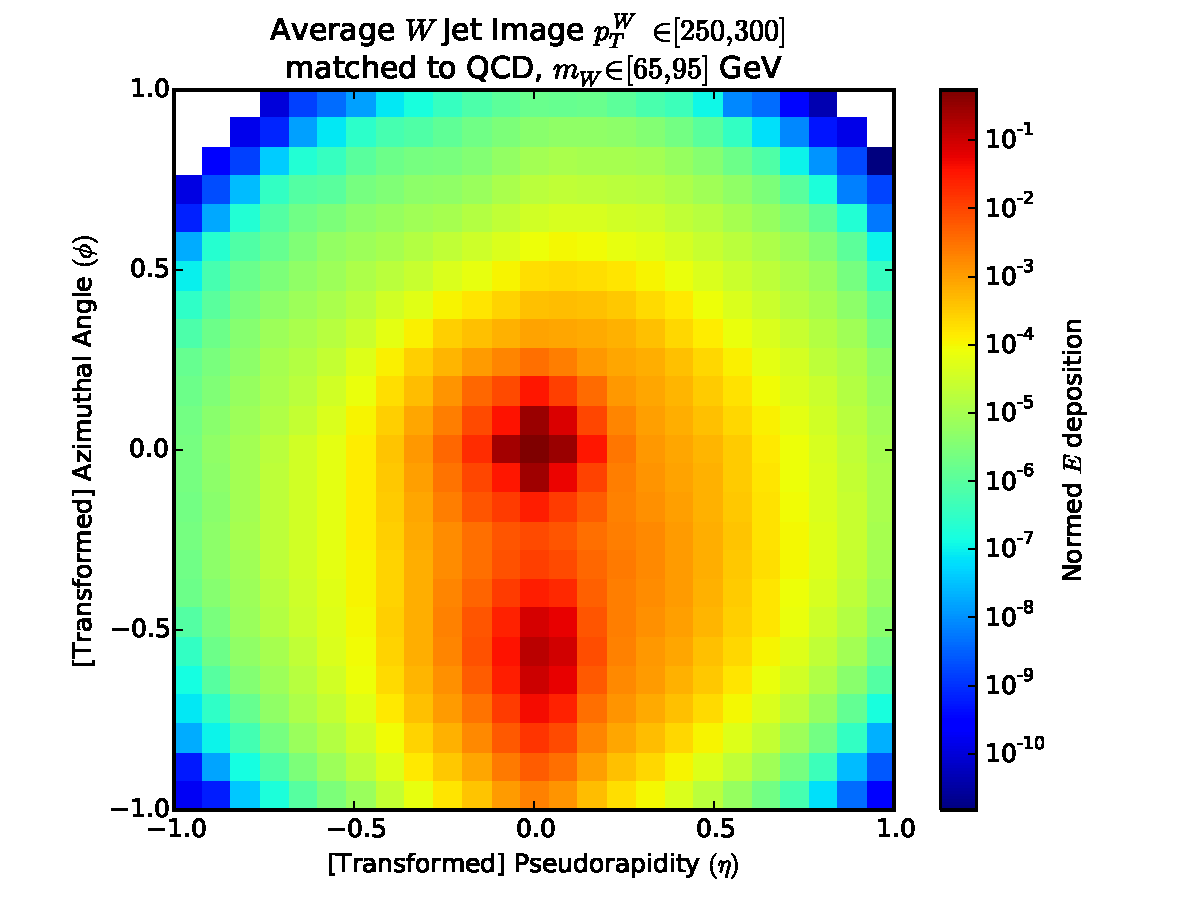
\includegraphics[width=0.5\textwidth]{figures/sig-im.pdf}
      }
      \subfloat[Average weighted QCD image \label{subfig:weighted_bkg}]{
        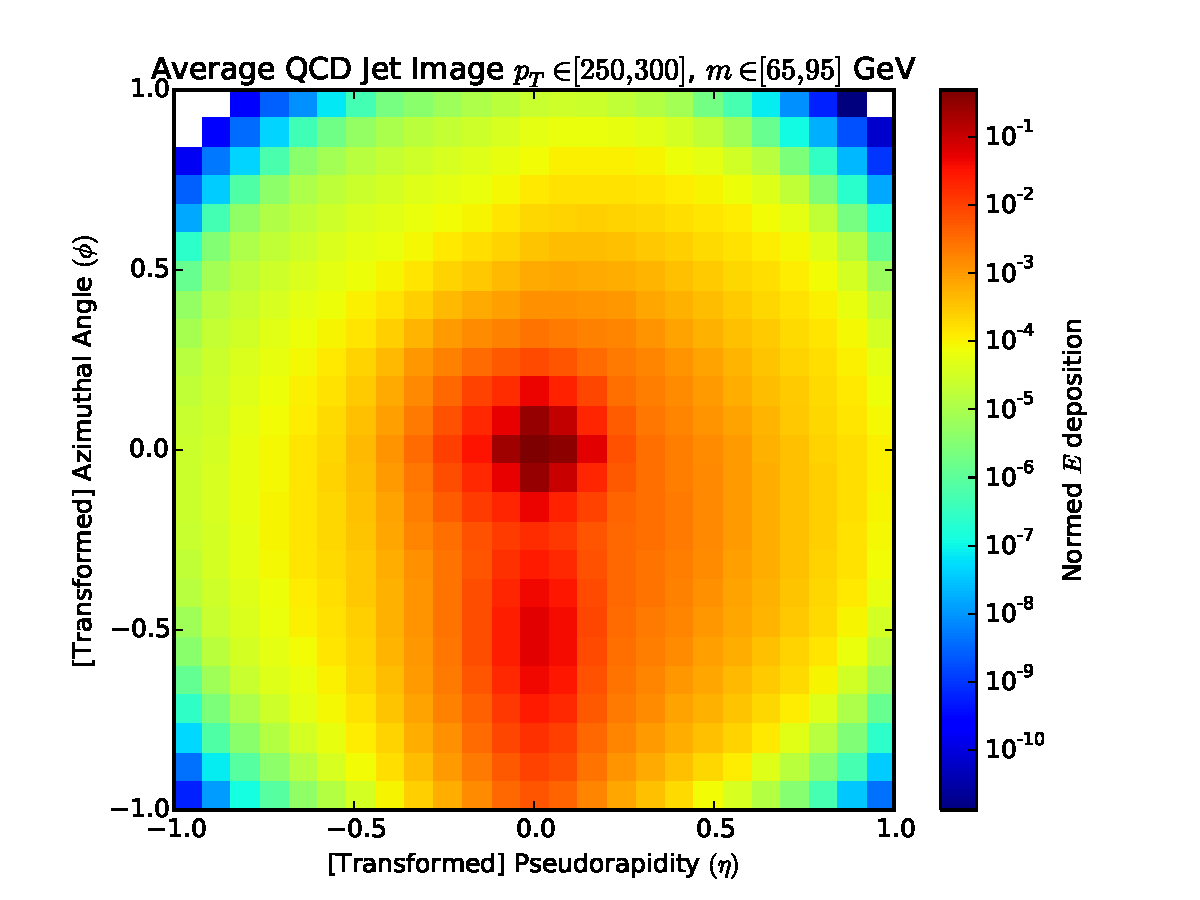
\includegraphics[width=0.5\textwidth]{figures/bkg-im.pdf}
      }
      \caption{Weighted $W'\rightarrow WZ$ (left) and QCD (right) average jet-image
      \label{fig:meanImages} }
    \end{center}
\end{figure}  


